\section{ادغام اشکال ها و تشکیل مجدد دیکشنری اشکال}
در این گام نیاز است که اشکالاتی که در مراحل قبل کشف شده‌اند، را ادغام کنیم. برای این منظور با توجه به این که اشکالات با هم معادل هستند(
\lr{Fault Collapsing}
)
، آن ها را با هم ادغام می‌کنیم.
\subsection{مشخص کردن اشکالات معادل}
در این گام نیاز است که اشکالات معادل را مشخص کنیم. برای این منظور مشابه با شکل زیر عمل می کنیم:
\\
\begin{figure}[H]
	\centering
	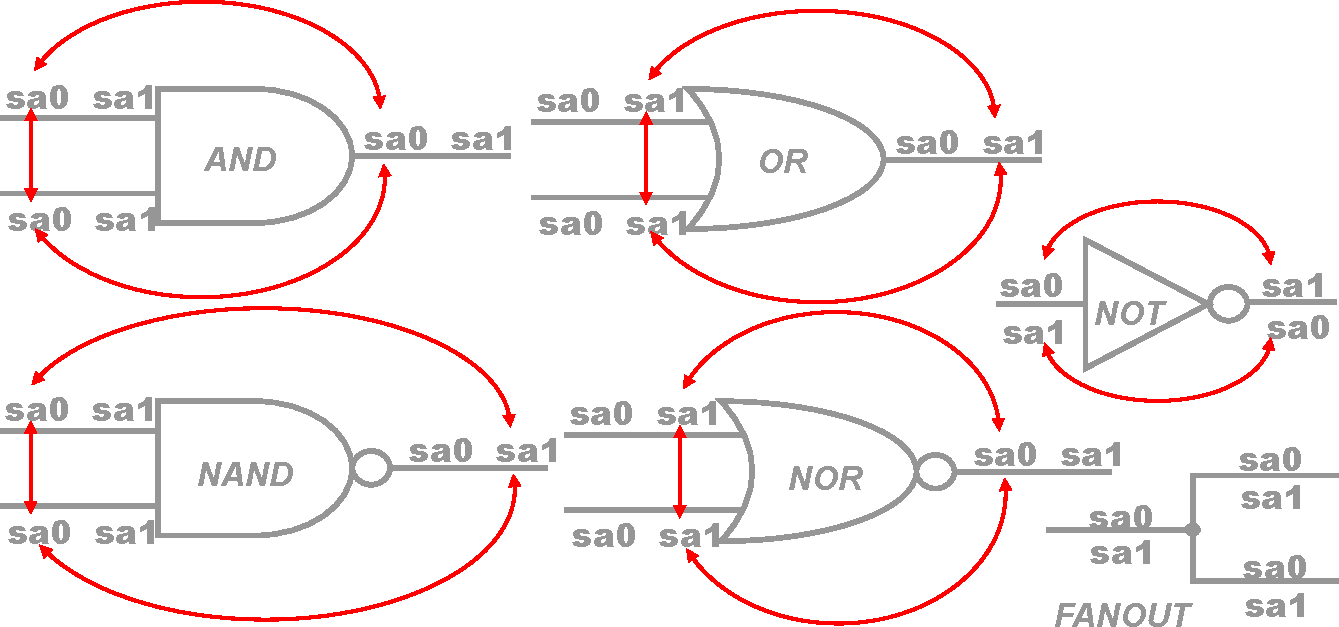
\includegraphics[scale=0.5]{fault_collapsing/images/fault_collapsing.pdf}
	\label{FaultCollapsing}
	\caption{چگونگی ادغام اشکال ها در هر گیت منطقی}
\end{figure}

کد نوشته شده برای این قسمت به شرح زیر است:
\small{
	\begin{latin}
		\begin{lstlisting}[numbers=left, breaklines=true,language=Python]
class FaultCollapseOperation(Operation):
	@classmethod
	def buffer_operation(cls, gate: BufferGate) -> list[tuple[str, list[str]]]:
	return [
		(
			f'{gate.output_wires[0].id}_s-a-0',
			[f'{gate.input_wires[0].id}_s-a-0']
		),
		(
			f'{gate.output_wires[0].id}_s-a-1',
			[f'{gate.input_wires[0].id}_s-a-1']
		),
	]
	
	@classmethod
	def not_operation(cls, gate: NotGate) -> list[tuple[str, list[str]]]:
	return [
		(
			f'{gate.output_wires[0].id}_s-a-0',
			[f'{gate.input_wires[0].id}_s-a-1']
		),
		(
			f'{gate.output_wires[0].id}_s-a-1',
			[f'{gate.input_wires[0].id}_s-a-0']
		),
	]
	
	@classmethod
	def and_operation(cls, gate: AndGate) -> list[tuple[str, list[str]]]:
	return [
		(
			f'{gate.output_wires[0].id}_s-a-0',
			[f'{input_wire.id}_s-a-0' for input_wire in gate.input_wires]
		),
	]
	
	@classmethod
	def or_operation(cls, gate: OrGate) -> list[tuple[str, list[str]]]:
	return [
		(
			f'{gate.output_wires[0].id}_s-a-1',
			[f'{input_wire.id}_s-a-1' for input_wire in gate.input_wires]
		)
	]
	
	@classmethod
	def nand_operation(cls, gate: NandGate) -> list[tuple[str, list[str]]]:
	return [
		(
			f'{gate.output_wires[0].id}_s-a-1',
			[f'{input_wire.id}_s-a-0' for input_wire in gate.input_wires]
		)
	]
	
	@classmethod
	def nor_operation(cls, gate: NorGate) -> list[tuple[str, list[str]]]:
		return [
		(
			f'{gate.output_wires[0].id}_s-a-0',
			[f'{input_wire.id}_s-a-1' for input_wire in gate.input_wires]
		)
		]
	
	@classmethod
	def xor_operation(cls, gate: XorGate) -> list[tuple[str, list[str]]]:
		return []
	
	@classmethod
	def xor_operation(cls, gate: XnorGate) -> list[tuple[str, list[str]]]:
		return []
	
	@classmethod
	def fanout_operation(cls, gate: FanoutGate) -> list[tuple[str, list[str]]]:
		return []
		\end{lstlisting}
	\end{latin}
}

همانطور که از کد بالا مشخص است، نیاز است خطاهای معادل هر خط ورودی گیت را در صورت لزوم مشخص کنیم. حال نیاز است، اشکالات معادل را بر مدار اعمال کنیم. برای این منظور از کد زیر زیر استفاده می کنیم:

\small{
	\begin{latin}
		\begin{lstlisting}[numbers=left, breaklines=true,language=Python]
def apply_fault_collapse(self) -> None:
	assert self.__equivalent_fault_dict

	for test_vector_bin, detected_faults in self.__detected_fault_dict.items():
		temp_detected_faults: list[str] = list(detected_faults)

	for gate_level in range(self.__network_controller.max_network_level):
	for _, gates in self.__network_controller.total_gates_with_level.items():
	for gate in gates:
	if not isinstance(gate, FanoutGate):
		for input_wire in gate.input_wires:
			s_a_0_fault: str = f'{input_wire.id}_s-a-0'
			s_a_1_fault: str = f'{input_wire.id}_s-a-1'
			
			if s_a_0_fault in temp_detected_faults:
				temp_detected_faults[temp_detected_faults.index(
					s_a_0_fault)
				] = self.__get_eqivalent_fault(fault_name=s_a_0_fault)

			if s_a_1_fault in temp_detected_faults:
				temp_detected_faults[temp_detected_faults.index(
					s_a_1_fault)
				] = self.__get_eqivalent_fault(fault_name=s_a_1_fault)

		self.__detected_fault_dict[test_vector_bin] = set(
			temp_detected_faults
		)
		\end{lstlisting}
	\end{latin}
}

\subsection{مشخص کردن بردار های تست ضروری}
همچنین نیاز است، بردار های تست ضروری
\LTRfootnote{Essential Test Vector}
 را نیز مشخص کنیم. روش کار به این صورت است که اگر یک اشکال توسط یک بردار شناسایی شود، آن بردار به صورت ضروری است. برای این منظور از تکه کد زیر استفاده می کنیم.
 
\small{
	\begin{latin}
		\begin{lstlisting}[numbers=left, breaklines=true,language=Python]
def essential_test_vectors(self) -> list[str]:
	detected_fault_test_vectors: dict[str: list[str]] = dict()
	for test_vector_bin, detected_faults in self.__detected_fault_dict.items():
		for detected_fault in detected_faults:
			if detected_fault not in detected_fault_test_vectors:
				detected_fault_test_vectors[detected_fault] = [test_vector_bin]
			else:
				detected_fault_test_vectors[detected_fault].append(test_vector_bin)

	essential_test_vectors_: list[str] = list()

	for _, test_vectors in detected_fault_test_vectors.items():
		if len(test_vectors) == 1:
			essential_test_vectors_.append(test_vectors[0])
	return essential_test_vectors_
		\end{lstlisting}
	\end{latin}
}

\subsection{تشکیل مجدد جدول اشکال}
پس از ادغام اشکالات، جدول اشکال به صورت زیر خواهد بود:

\begin{table}[H]
\centering
\begin{latin}
\scalebox{0.3}{
	\begin{tabular}{|c|c|c|c|c|c|c|c|c|c|c|c|c|c|c|c|c|c|c|c|c|c|c|c|}
		\hline
		test vector & 3\_2\_s-a-1 & 16\_s-a-1 & 11\_s-a-1 & 16\_1\_s-a-1 & 3\_s-a-0 & 11\_1\_s-a-1 & 11\_s-a-0 & 19\_s-a-1 & 3\_s-a-1 & 10\_s-a-1 & 11\_2\_s-a-1 & 2\_s-a-1 & 1\_s-a-1 & 16\_2\_s-a-1 & 23\_s-a-1 & 22\_s-a-0 & 3\_1\_s-a-1 & 6\_s-a-1 & 7\_s-a-1 & 23\_s-a-0 & 16\_s-a-0 & 22\_s-a-1 & Essential / Not Essential \\ \hline
		00000 & ~ & ~ & ~ & ~ & ~ & ~ & ~ & ~ & ~ & ~ & ~ & Y & ~ & ~ & Y & ~ & ~ & ~ & Y & ~ & Y & Y & Not Essential \\ \hline
		00001 & ~ & ~ & ~ & ~ & ~ & ~ & Y & Y & ~ & ~ & ~ & Y & ~ & ~ & ~ & ~ & ~ & ~ & ~ & Y & Y & Y & Not Essential \\ \hline
		00010 & ~ & ~ & ~ & ~ & ~ & ~ & ~ & ~ & ~ & ~ & ~ & Y & ~ & ~ & Y & ~ & ~ & ~ & Y & ~ & Y & Y & Not Essential \\ \hline
		00011 & Y & ~ & ~ & ~ & ~ & ~ & Y & Y & Y & ~ & ~ & Y & ~ & ~ & ~ & ~ & ~ & ~ & ~ & Y & Y & Y & Not Essential \\ \hline
		00100 & ~ & ~ & ~ & ~ & ~ & ~ & ~ & ~ & ~ & ~ & ~ & Y & Y & ~ & Y & ~ & ~ & ~ & Y & ~ & Y & Y & Not Essential \\ \hline
		00101 & ~ & ~ & ~ & ~ & ~ & ~ & Y & Y & ~ & ~ & ~ & Y & Y & ~ & ~ & ~ & ~ & Y & ~ & Y & Y & Y & Not Essential \\ \hline
		00110 & ~ & ~ & ~ & ~ & ~ & ~ & ~ & ~ & ~ & ~ & ~ & ~ & Y & ~ & Y & ~ & ~ & ~ & ~ & ~ & Y & Y & Not Essential \\ \hline
		00111 & ~ & ~ & Y & ~ & Y & ~ & ~ & ~ & ~ & ~ & Y & ~ & Y & ~ & Y & ~ & ~ & ~ & ~ & ~ & Y & Y & Not Essential \\ \hline
		01000 & ~ & Y & ~ & Y & ~ & ~ & Y & ~ & ~ & ~ & ~ & ~ & ~ & Y & ~ & Y & ~ & ~ & ~ & Y & ~ & ~ & Not Essential \\ \hline
		01001 & ~ & Y & ~ & Y & ~ & ~ & Y & ~ & ~ & ~ & ~ & ~ & ~ & ~ & ~ & Y & ~ & ~ & ~ & Y & ~ & ~ & Not Essential \\ \hline
		01010 & Y & Y & ~ & Y & ~ & ~ & Y & ~ & Y & ~ & ~ & ~ & ~ & Y & ~ & Y & ~ & ~ & ~ & Y & ~ & ~ & Not Essential \\ \hline
		01011 & Y & Y & ~ & Y & ~ & ~ & Y & ~ & Y & ~ & ~ & ~ & ~ & ~ & ~ & Y & ~ & ~ & ~ & Y & ~ & ~ & Not Essential \\ \hline
		01100 & ~ & Y & ~ & Y & ~ & ~ & Y & ~ & ~ & ~ & ~ & ~ & ~ & Y & ~ & Y & ~ & Y & ~ & Y & ~ & ~ & Not Essential \\ \hline
		01101 & ~ & Y & ~ & Y & ~ & ~ & Y & ~ & ~ & ~ & ~ & ~ & ~ & ~ & ~ & Y & ~ & Y & ~ & Y & ~ & ~ & Not Essential \\ \hline
		01110 & ~ & ~ & Y & ~ & Y & Y & ~ & ~ & ~ & ~ & ~ & ~ & Y & ~ & Y & ~ & ~ & ~ & ~ & ~ & Y & Y & Not Essential \\ \hline
		01111 & ~ & ~ & Y & ~ & Y & Y & ~ & ~ & ~ & ~ & Y & ~ & Y & ~ & Y & ~ & ~ & ~ & ~ & ~ & Y & Y & Not Essential \\ \hline
		10000 & ~ & ~ & ~ & ~ & ~ & ~ & ~ & ~ & Y & ~ & ~ & Y & ~ & ~ & Y & ~ & Y & ~ & Y & ~ & Y & Y & Not Essential \\ \hline
		10001 & ~ & ~ & ~ & ~ & ~ & ~ & Y & Y & Y & ~ & ~ & Y & ~ & ~ & ~ & ~ & Y & ~ & ~ & Y & Y & Y & Not Essential \\ \hline
		10010 & ~ & ~ & ~ & ~ & ~ & ~ & ~ & ~ & Y & ~ & ~ & Y & ~ & ~ & Y & ~ & Y & ~ & Y & ~ & Y & Y & Not Essential \\ \hline
		10011 & Y & ~ & ~ & ~ & ~ & ~ & Y & Y & Y & ~ & ~ & Y & ~ & ~ & ~ & ~ & Y & ~ & ~ & Y & Y & Y & Not Essential \\ \hline
		10100 & ~ & ~ & ~ & ~ & Y & ~ & ~ & ~ & ~ & Y & ~ & Y & ~ & ~ & Y & Y & ~ & ~ & Y & ~ & Y & ~ & Not Essential \\ \hline
		10101 & ~ & ~ & ~ & ~ & Y & ~ & Y & Y & ~ & Y & ~ & ~ & ~ & ~ & ~ & Y & ~ & Y & ~ & Y & ~ & ~ & Not Essential \\ \hline
		10110 & ~ & ~ & ~ & ~ & Y & ~ & ~ & ~ & ~ & Y & ~ & ~ & ~ & ~ & Y & Y & ~ & ~ & ~ & ~ & Y & ~ & Not Essential \\ \hline
		10111 & ~ & ~ & Y & ~ & Y & ~ & ~ & ~ & ~ & Y & Y & ~ & ~ & ~ & Y & Y & ~ & ~ & ~ & ~ & Y & ~ & Not Essential \\ \hline
		11000 & ~ & Y & ~ & Y & ~ & ~ & Y & ~ & ~ & ~ & ~ & ~ & ~ & Y & ~ & Y & ~ & ~ & ~ & Y & ~ & ~ & Not Essential \\ \hline
		11001 & ~ & Y & ~ & Y & ~ & ~ & Y & ~ & ~ & ~ & ~ & ~ & ~ & ~ & ~ & Y & ~ & ~ & ~ & Y & ~ & ~ & Not Essential \\ \hline
		11010 & Y & Y & ~ & Y & ~ & ~ & Y & ~ & Y & ~ & ~ & ~ & ~ & Y & ~ & Y & ~ & ~ & ~ & Y & ~ & ~ & Not Essential \\ \hline
		11011 & Y & Y & ~ & Y & ~ & ~ & Y & ~ & Y & ~ & ~ & ~ & ~ & ~ & ~ & Y & ~ & ~ & ~ & Y & ~ & ~ & Not Essential \\ \hline
		11100 & ~ & Y & ~ & ~ & ~ & ~ & Y & ~ & ~ & ~ & ~ & ~ & ~ & Y & ~ & Y & ~ & Y & ~ & Y & ~ & ~ & Not Essential \\ \hline
		11101 & ~ & ~ & ~ & ~ & ~ & ~ & Y & ~ & ~ & ~ & ~ & ~ & ~ & ~ & ~ & Y & ~ & Y & ~ & Y & ~ & ~ & Not Essential \\ \hline
		11110 & ~ & ~ & Y & ~ & Y & Y & ~ & ~ & ~ & Y & ~ & ~ & ~ & ~ & Y & Y & ~ & ~ & ~ & ~ & Y & ~ & Not Essential \\ \hline
		11111 & ~ & ~ & Y & ~ & Y & Y & ~ & ~ & ~ & Y & Y & ~ & ~ & ~ & Y & Y & ~ & ~ & ~ & ~ & Y & ~ & Not Essential \\ \hline
	\end{tabular}
}
\end{latin}
\caption{جدول اشکال \lr{c17} پس از ادغام اشکالات}
\end{table}